\documentclass{beamer}
\usetheme{Madrid}
\usefonttheme{serif}

% Here are the packages I use for equations, code, inserting images, making graphs, and dark mode document, basically.

\usepackage{amsmath}
\usepackage{listings}
\lstset{
    basicstyle=\small\ttfamily,
    breaklines=true
}
\usepackage{graphicx}

\AtBeginSection[]
{
  \begin{frame}
    \frametitle{Table of Contents}
    \tableofcontents[currentsection]
  \end{frame}
}

\title{Analysis of Block Matching Algorithms for Image Transformation}
\subtitle{ADA Final Project: Questions 5 - 10}
\author{Alejandro Goicochea\and Diego Linares\and Ariana Villegas}
\institute{\inst{}Universidad de Ingeniería y Tecnología}
\date{July 23, 2020}

\begin{document}
  \frame{\titlepage}
  \begin{frame}
    \frametitle{Table of Contents}
    \tableofcontents
  \end{frame}
  \section{Recap of Block Matching}
    \begin{frame}
      \frametitle{Previous Presentation}
      In the previous presentation we designed \textbf{two algorithms} for block matching:
      \begin{itemize}
        \item Greedy / Naive Algorithm
        \item Memoized Algorithm (now improved to DP version).
      \end{itemize}
      \medskip
      For this last part we are including a third algorithm, a DP with \textbf{better weight}.\\
      \medskip
      We are gonna see how each of this performs for image transformation. 
    \end{frame}
    
    \begin{frame}
      \frametitle{Greedy Algorithm}
      
      \begin{figure}
		\centering
		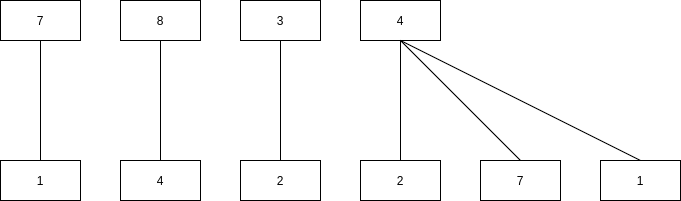
\includegraphics[scale=.48]{greedy.png}
		\caption{Greedy Algorithm}
		\label{fig:greedy_algorithm}
	  \end{figure}
      
    \end{frame}
    
    \begin{frame}
      \frametitle{Recursion}
      
      \begin{figure}
		\centering
		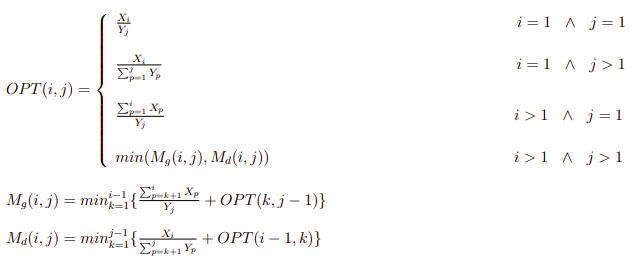
\includegraphics[scale=.48]{recursion.png}
		\caption{Recursion}
		\label{fig:Recursion}
	  \end{figure}
      
    \end{frame}
    
    \begin{frame}
      \frametitle{Dynamic Programming Algorithm}
      
      \begin{figure}
		\centering
		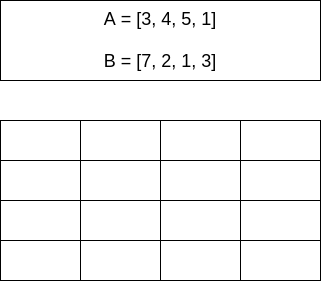
\includegraphics[scale=.48]{dp_0.png}
		\caption{Dynamic Programming Algorithm - Initial}
		\label{fig:dynamic_programming_algorithm_0}
	  \end{figure}
      
    \end{frame}
    
    \begin{frame}
      \frametitle{Dynamic Programming Algorithm}
      
      \begin{figure}
		\centering
		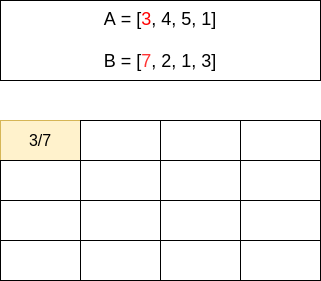
\includegraphics[scale=.48]{dp_1.png}
		\caption{Dynamic Programming Algorithm - Step 1}
		\label{fig:dynamic_programming_algorithm_1}
	  \end{figure}
      
    \end{frame}
    
    \begin{frame}
      \frametitle{Dynamic Programming Algorithm}
      
      \begin{figure}
		\centering
		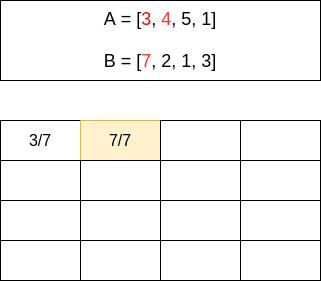
\includegraphics[scale=.48]{dp_2.png}
		\caption{Dynamic Programming Algorithm - Step 1}
		\label{fig:dynamic_programming_algorithm_2}
	  \end{figure}
      
    \end{frame}
    
    \begin{frame}
      \frametitle{Dynamic Programming Algorithm}
      
      \begin{figure}
		\centering
		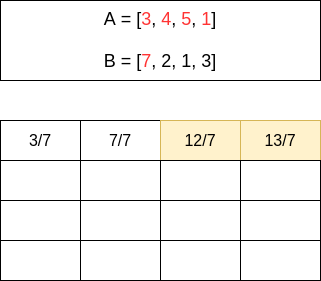
\includegraphics[scale=.48]{dp_3.png}
		\caption{Dynamic Programming Algorithm - Step 1}
		\label{fig:dynamic_programming_algorithm_3}
	  \end{figure}
      
    \end{frame}
    
    \begin{frame}
      \frametitle{Dynamic Programming Algorithm}
      
      \begin{figure}
		\centering
		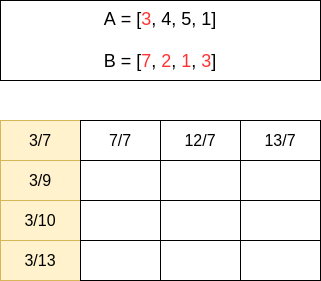
\includegraphics[scale=.48]{dp_4.png}
		\caption{Dynamic Programming Algorithm - Step 2}
		\label{fig:dynamic_programming_algorithm_4}
	  \end{figure}
      
    \end{frame}
    
    \begin{frame}
      \frametitle{Dynamic Programming Algorithm}
      
      \begin{figure}
		\centering
		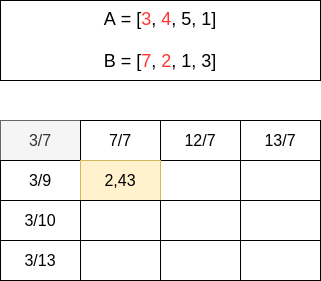
\includegraphics[scale=.48]{dp_5.png}
		\caption{Dynamic Programming Algorithm - Step 3}
		\label{fig:dynamic_programming_algorithm_5}
	  \end{figure}
      
    \end{frame}
    
    \begin{frame}
      \frametitle{Dynamic Programming Algorithm}
      
      \begin{figure}
		\centering
		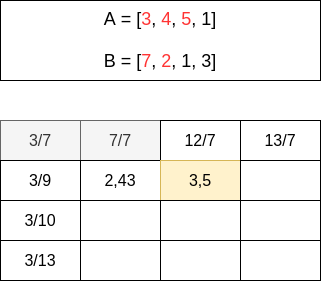
\includegraphics[scale=.48]{dp_6.png}
		\caption{Dynamic Programming Algorithm - Step 3}
		\label{fig:dynamic_programming_algorithm_6}
	  \end{figure}
      
    \end{frame}
    
    \begin{frame}
      \frametitle{Dynamic Programming Algorithm}
      
      \begin{figure}
		\centering
		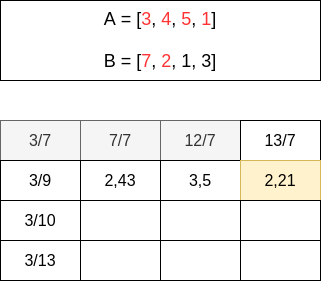
\includegraphics[scale=.48]{dp_7.png}
		\caption{Dynamic Programming Algorithm - Step 3}
		\label{fig:dynamic_programming_algorithm_7}
	  \end{figure}
      
    \end{frame}
    
    \begin{frame}
      \frametitle{Dynamic Programming Algorithm}
      
      \begin{figure}
		\centering
		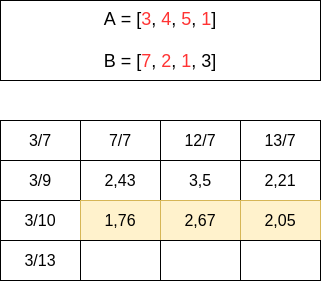
\includegraphics[scale=.48]{dp_8.png}
		\caption{Dynamic Programming Algorithm - Step 4}
		\label{fig:dynamic_programming_algorithm_8}
	  \end{figure}
      
    \end{frame}
    
    \begin{frame}
      \frametitle{Dynamic Programming Algorithm}
      
      \begin{figure}
		\centering
		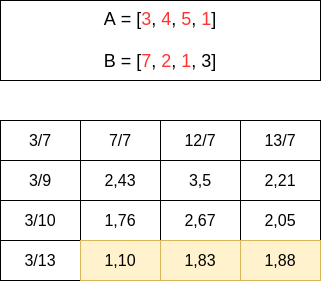
\includegraphics[scale=.48]{dp_9.png}
		\caption{Dynamic Programming Algorithm - Step 5}
		\label{fig:dynamic_programming_algorithm_9}
	  \end{figure}
      
    \end{frame}
    
  \section{Decoding Images through Luma}
    \subsection{What is Luma?}
    \subsection{Transforming into a Matrix of bits}
  \section{Our Approach}
    \subsection{Base Process for Transformation}
    \subsection{Different Algorithms}
  \section{Examples}
  \section{Conclusion}
    \subsection{Algorithm Effectiveness}
    \subsection{Personal Valoration}

\end{document}